\begin{tikzpicture}
\node[anchor=south west,inner sep=0] at (0,0) {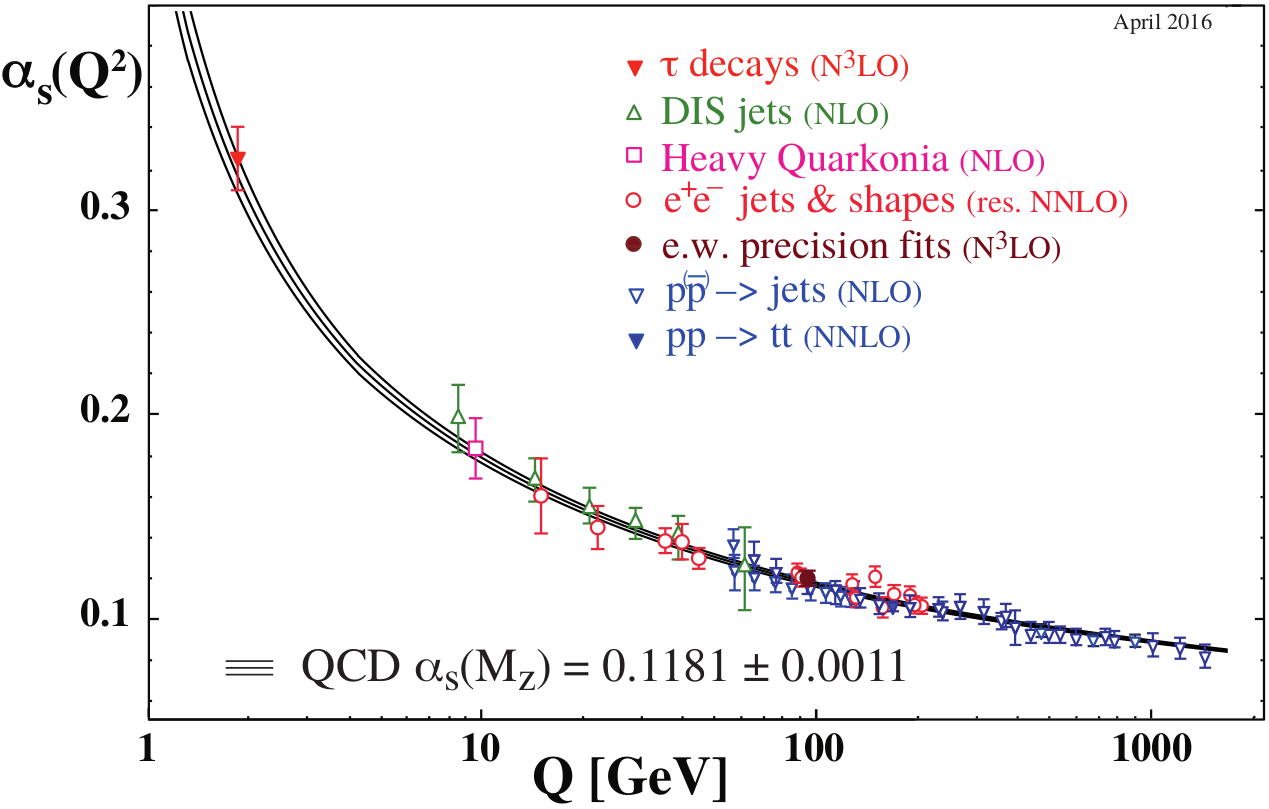
\includegraphics[width=10cm]{\PhDthesisdir/plots_and_images/from_PDG_booklet_2018/QCD_value_fct_Q.png}};
\fill [white] (1,0) rectangle (10, .65);
\fill [white] (1.15,0) rectangle (0,6);
\fill [white] (1.5,.85) rectangle (7.2,1.3);

\draw (1.2,.5) node {\small \num{1}} ;
\draw (3.8,.5) node {\small \num{10}} ;
\draw (6.45,.5) node {\small \num{100}} ;
\draw (9.1,.5) node {\small \num{1000}} ;

\draw (5,.25) node {$k$ (\SI{}{\GeV})} ;

\draw (.8,1.5) node {\small \num{0.1}} ;
\draw (.8,3.15) node {\small \num{0.2}} ;
\draw (.8,4.7) node {\small \num{0.3}} ;

\draw (.5,5.8) node {$\alpha_s(k)$} ;

\draw (1.6, 1.1) node [right] {\small $\equiv$ QCD $\alpha_s(m_{\Zboson}) = \num{0.1181}\pm\num{0.0011}$};
\end{tikzpicture}
